\documentclass[1p]{elsarticle_modified}
%\bibliographystyle{elsarticle-num}

%\usepackage[colorlinks]{hyperref}
%\usepackage{abbrmath_seonhwa} %\Abb, \Ascr, \Acal ,\Abf, \Afrak
\usepackage{amsfonts}
\usepackage{amssymb}
\usepackage{amsmath}
\usepackage{amsthm}
\usepackage{scalefnt}
\usepackage{amsbsy}
\usepackage{kotex}
\usepackage{caption}
\usepackage{subfig}
\usepackage{color}
\usepackage{graphicx}
\usepackage{xcolor} %% white, black, red, green, blue, cyan, magenta, yellow
\usepackage{float}
\usepackage{setspace}
\usepackage{hyperref}

\usepackage{tikz}
\usetikzlibrary{arrows}

\usepackage{multirow}
\usepackage{array} % fixed length table
\usepackage{hhline}

%%%%%%%%%%%%%%%%%%%%%
\makeatletter
\renewcommand*\env@matrix[1][\arraystretch]{%
	\edef\arraystretch{#1}%
	\hskip -\arraycolsep
	\let\@ifnextchar\new@ifnextchar
	\array{*\c@MaxMatrixCols c}}
\makeatother %https://tex.stackexchange.com/questions/14071/how-can-i-increase-the-line-spacing-in-a-matrix
%%%%%%%%%%%%%%%

\usepackage[normalem]{ulem}

\newcommand{\msout}[1]{\ifmmode\text{\sout{\ensuremath{#1}}}\else\sout{#1}\fi}
%SOURCE: \msout is \stkout macro in https://tex.stackexchange.com/questions/20609/strikeout-in-math-mode

\newcommand{\cancel}[1]{
	\ifmmode
	{\color{red}\msout{#1}}
	\else
	{\color{red}\sout{#1}}
	\fi
}

\newcommand{\add}[1]{
	{\color{blue}\uwave{#1}}
}

\newcommand{\replace}[2]{
	\ifmmode
	{\color{red}\msout{#1}}{\color{blue}\uwave{#2}}
	\else
	{\color{red}\sout{#1}}{\color{blue}\uwave{#2}}
	\fi
}

\newcommand{\Sol}{\mathcal{S}} %segment
\newcommand{\D}{D} %diagram
\newcommand{\A}{\mathcal{A}} %arc


%%%%%%%%%%%%%%%%%%%%%%%%%%%%%5 test

\def\sl{\operatorname{\textup{SL}}(2,\Cbb)}
\def\psl{\operatorname{\textup{PSL}}(2,\Cbb)}
\def\quan{\mkern 1mu \triangleright \mkern 1mu}

\theoremstyle{definition}
\newtheorem{thm}{Theorem}[section]
\newtheorem{prop}[thm]{Proposition}
\newtheorem{lem}[thm]{Lemma}
\newtheorem{ques}[thm]{Question}
\newtheorem{cor}[thm]{Corollary}
\newtheorem{defn}[thm]{Definition}
\newtheorem{exam}[thm]{Example}
\newtheorem{rmk}[thm]{Remark}
\newtheorem{alg}[thm]{Algorithm}

\newcommand{\I}{\sqrt{-1}}
\begin{document}

%\begin{frontmatter}
%
%\title{Boundary parabolic representations of knots up to 8 crossings}
%
%%% Group authors per affiliation:
%\author{Yunhi Cho} 
%\address{Department of Mathematics, University of Seoul, Seoul, Korea}
%\ead{yhcho@uos.ac.kr}
%
%
%\author{Seonhwa Kim} %\fnref{s_kim}}
%\address{Center for Geometry and Physics, Institute for Basic Science, Pohang, 37673, Korea}
%\ead{ryeona17@ibs.re.kr}
%
%\author{Hyuk Kim}
%\address{Department of Mathematical Sciences, Seoul National University, Seoul 08826, Korea}
%\ead{hyukkim@snu.ac.kr}
%
%\author{Seokbeom Yoon}
%\address{Department of Mathematical Sciences, Seoul National University, Seoul, 08826,  Korea}
%\ead{sbyoon15@snu.ac.kr}
%
%\begin{abstract}
%We find all boundary parabolic representation of knots up to 8 crossings.
%
%\end{abstract}
%\begin{keyword}
%    \MSC[2010] 57M25 
%\end{keyword}
%
%\end{frontmatter}

%\linenumbers
%\tableofcontents
%
\newcommand\colored[1]{\textcolor{white}{\rule[-0.35ex]{0.8em}{1.4ex}}\kern-0.8em\color{red} #1}%
%\newcommand\colored[1]{\textcolor{white}{ #1}\kern-2.17ex	\textcolor{white}{ #1}\kern-1.81ex	\textcolor{white}{ #1}\kern-2.15ex\color{red}#1	}

{\Large $\underline{12a_{1018}~(K12a_{1018})}$}

\setlength{\tabcolsep}{10pt}
\renewcommand{\arraystretch}{1.6}
\vspace{1cm}\begin{tabular}{m{100pt}>{\centering\arraybackslash}m{274pt}}
\multirow{5}{120pt}{
	\centering
	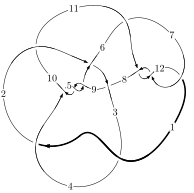
\includegraphics[width=112pt]{../../../GIT/diagram.site/Diagrams/png/1819_12a_1018.png}\\
\ \ \ A knot diagram\footnotemark}&
\allowdisplaybreaks
\textbf{Linearized knot diagam} \\
\cline{2-2}
 &
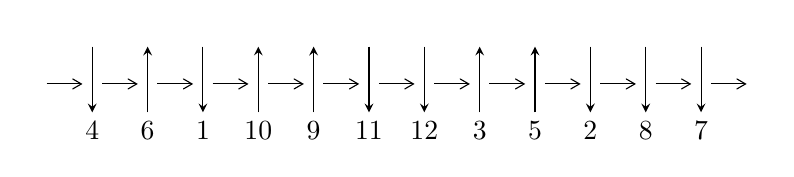
\begin{tikzpicture}[x=20pt, y=17pt]
	% nodes
	\node (C0) at (0, 0) {};
	\node (C1) at (1, 0) {};
	\node (C1U) at (1, +1) {};
	\node (C1D) at (1, -1) {4};

	\node (C2) at (2, 0) {};
	\node (C2U) at (2, +1) {};
	\node (C2D) at (2, -1) {6};

	\node (C3) at (3, 0) {};
	\node (C3U) at (3, +1) {};
	\node (C3D) at (3, -1) {1};

	\node (C4) at (4, 0) {};
	\node (C4U) at (4, +1) {};
	\node (C4D) at (4, -1) {10};

	\node (C5) at (5, 0) {};
	\node (C5U) at (5, +1) {};
	\node (C5D) at (5, -1) {9};

	\node (C6) at (6, 0) {};
	\node (C6U) at (6, +1) {};
	\node (C6D) at (6, -1) {11};

	\node (C7) at (7, 0) {};
	\node (C7U) at (7, +1) {};
	\node (C7D) at (7, -1) {12};

	\node (C8) at (8, 0) {};
	\node (C8U) at (8, +1) {};
	\node (C8D) at (8, -1) {3};

	\node (C9) at (9, 0) {};
	\node (C9U) at (9, +1) {};
	\node (C9D) at (9, -1) {5};

	\node (C10) at (10, 0) {};
	\node (C10U) at (10, +1) {};
	\node (C10D) at (10, -1) {2};

	\node (C11) at (11, 0) {};
	\node (C11U) at (11, +1) {};
	\node (C11D) at (11, -1) {8};

	\node (C12) at (12, 0) {};
	\node (C12U) at (12, +1) {};
	\node (C12D) at (12, -1) {7};
	\node (C13) at (13, 0) {};

	% arrows
	\draw[->,>={angle 60}]
	(C0) edge (C1) (C1) edge (C2) (C2) edge (C3) (C3) edge (C4) (C4) edge (C5) (C5) edge (C6) (C6) edge (C7) (C7) edge (C8) (C8) edge (C9) (C9) edge (C10) (C10) edge (C11) (C11) edge (C12) (C12) edge (C13) ;	\draw[->,>=stealth]
	(C1U) edge (C1D) (C2D) edge (C2U) (C3U) edge (C3D) (C4D) edge (C4U) (C5D) edge (C5U) (C6U) edge (C6D) (C7U) edge (C7D) (C8D) edge (C8U) (C9D) edge (C9U) (C10U) edge (C10D) (C11U) edge (C11D) (C12U) edge (C12D) ;
	\end{tikzpicture} \\
\hhline{~~} \\& 
\textbf{Solving Sequence} \\ \cline{2-2} 
 &
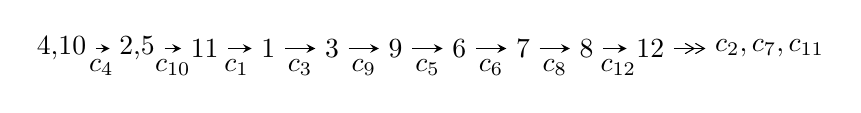
\begin{tikzpicture}[x=23pt, y=7pt]
	% node
	\node (A0) at (-1/8, 0) {4,10};
	\node (A1) at (17/16, 0) {2,5};
	\node (A2) at (17/8, 0) {11};
	\node (A3) at (25/8, 0) {1};
	\node (A4) at (33/8, 0) {3};
	\node (A5) at (41/8, 0) {9};
	\node (A6) at (49/8, 0) {6};
	\node (A7) at (57/8, 0) {7};
	\node (A8) at (65/8, 0) {8};
	\node (A9) at (73/8, 0) {12};
	\node (C1) at (1/2, -1) {$c_{4}$};
	\node (C2) at (13/8, -1) {$c_{10}$};
	\node (C3) at (21/8, -1) {$c_{1}$};
	\node (C4) at (29/8, -1) {$c_{3}$};
	\node (C5) at (37/8, -1) {$c_{9}$};
	\node (C6) at (45/8, -1) {$c_{5}$};
	\node (C7) at (53/8, -1) {$c_{6}$};
	\node (C8) at (61/8, -1) {$c_{8}$};
	\node (C9) at (69/8, -1) {$c_{12}$};
	\node (A10) at (11, 0) {$c_{2},c_{7},c_{11}$};

	% edge
	\draw[->,>=stealth]	
	(A0) edge (A1) (A1) edge (A2) (A2) edge (A3) (A3) edge (A4) (A4) edge (A5) (A5) edge (A6) (A6) edge (A7) (A7) edge (A8) (A8) edge (A9) ;
	\draw[->>,>={angle 60}]	
	(A9) edge (A10);
\end{tikzpicture} \\ 

\end{tabular} \\

\footnotetext{
The image of knot diagram is generated by the software ``\textbf{Draw programme}" developed by Andrew Bartholomew(\url{http://www.layer8.co.uk/maths/draw/index.htm\#Running-draw}), where we modified some parts for our purpose(\url{https://github.com/CATsTAILs/LinksPainter}).
}\phantom \\ \newline 
\centering \textbf{Ideals for irreducible components\footnotemark of $X_{\text{par}}$} 
 
\begin{align*}
I^u_{1}&=\langle 
-8.80811\times10^{120} u^{82}-3.74088\times10^{121} u^{81}+\cdots+1.73742\times10^{122} b+3.18684\times10^{122},\\
\phantom{I^u_{1}}&\phantom{= \langle  }-6.10199\times10^{123} u^{82}+1.07219\times10^{124} u^{81}+\cdots+2.95362\times10^{123} a-9.13225\times10^{123},\\
\phantom{I^u_{1}}&\phantom{= \langle  }u^{83}-2 u^{82}+\cdots+2 u-1\rangle \\
I^u_{2}&=\langle 
b+1,\;- u^3+11 u^2+17 a-9 u+5,\;u^4- u^3+u^2+1\rangle \\
\\
\end{align*}
\raggedright * 2 irreducible components of $\dim_{\mathbb{C}}=0$, with total 87 representations.\\
\footnotetext{All coefficients of polynomials are rational numbers. But the coefficients are sometimes approximated in decimal forms when there is not enough margin.}
\newpage
\renewcommand{\arraystretch}{1}
\centering \section*{I. $I^u_{1}= \langle -8.81\times10^{120} u^{82}-3.74\times10^{121} u^{81}+\cdots+1.74\times10^{122} b+3.19\times10^{122},\;-6.10\times10^{123} u^{82}+1.07\times10^{124} u^{81}+\cdots+2.95\times10^{123} a-9.13\times10^{123},\;u^{83}-2 u^{82}+\cdots+2 u-1 \rangle$}
\flushleft \textbf{(i) Arc colorings}\\
\begin{tabular}{m{7pt} m{180pt} m{7pt} m{180pt} }
\flushright $a_{4}=$&$\begin{pmatrix}1\\0\end{pmatrix}$ \\
\flushright $a_{10}=$&$\begin{pmatrix}0\\u\end{pmatrix}$ \\
\flushright $a_{2}=$&$\begin{pmatrix}2.06594 u^{82}-3.63008 u^{81}+\cdots+1.45256 u+3.09189\\0.0506964 u^{82}+0.215312 u^{81}+\cdots-0.518239 u-1.83424\end{pmatrix}$ \\
\flushright $a_{5}=$&$\begin{pmatrix}1\\- u^2\end{pmatrix}$ \\
\flushright $a_{11}=$&$\begin{pmatrix}-2.65834 u^{82}+5.40550 u^{81}+\cdots+3.14748 u-8.59296\\0.367078 u^{82}-1.09517 u^{81}+\cdots+0.336880 u+1.82664\end{pmatrix}$ \\
\flushright $a_{1}=$&$\begin{pmatrix}2.11663 u^{82}-3.41477 u^{81}+\cdots+0.934318 u+1.25765\\0.0506964 u^{82}+0.215312 u^{81}+\cdots-0.518239 u-1.83424\end{pmatrix}$ \\
\flushright $a_{3}=$&$\begin{pmatrix}1.68022 u^{82}-2.87266 u^{81}+\cdots+2.28099 u+2.27888\\-0.146416 u^{82}+0.413543 u^{81}+\cdots+0.0785799 u-1.71128\end{pmatrix}$ \\
\flushright $a_{9}=$&$\begin{pmatrix}- u\\u^3+u\end{pmatrix}$ \\
\flushright $a_{6}=$&$\begin{pmatrix}u^2+1\\- u^4-2 u^2\end{pmatrix}$ \\
\flushright $a_{7}=$&$\begin{pmatrix}0.532917 u^{82}-0.701603 u^{81}+\cdots+1.65138 u+3.72914\\0.144848 u^{82}-0.280506 u^{81}+\cdots+0.0803900 u+0.0568371\end{pmatrix}$ \\
\flushright $a_{8}=$&$\begin{pmatrix}-0.858192 u^{82}+1.37862 u^{81}+\cdots-7.54635 u-4.74270\\0.321807 u^{82}-0.770401 u^{81}+\cdots-0.119629 u+0.879748\end{pmatrix}$ \\
\flushright $a_{12}=$&$\begin{pmatrix}-2.24967 u^{82}+4.84113 u^{81}+\cdots+6.28939 u-7.92112\\0.114212 u^{82}-0.200029 u^{81}+\cdots+1.38569 u-0.0353137\end{pmatrix}$\\&\end{tabular}
\flushleft \textbf{(ii) Obstruction class $= -1$}\\~\\
\flushleft \textbf{(iii) Cusp Shapes $= 4.42394 u^{82}-7.99659 u^{81}+\cdots-18.0819 u+5.80601$}\\~\\
\newpage\renewcommand{\arraystretch}{1}
\flushleft \textbf{(iv) u-Polynomials at the component}\newline \\
\begin{tabular}{m{50pt}|m{274pt}}
Crossings & \hspace{64pt}u-Polynomials at each crossing \\
\hline $$\begin{aligned}c_{1},c_{3}\end{aligned}$$&$\begin{aligned}
&u^{83}-5 u^{82}+\cdots+1900 u+289
\end{aligned}$\\
\hline $$\begin{aligned}c_{2}\end{aligned}$$&$\begin{aligned}
&u^{83}-7 u^{82}+\cdots-9656 u-4624
\end{aligned}$\\
\hline $$\begin{aligned}c_{4},c_{5},c_{9}\end{aligned}$$&$\begin{aligned}
&u^{83}-2 u^{82}+\cdots+2 u-1
\end{aligned}$\\
\hline $$\begin{aligned}c_{6}\end{aligned}$$&$\begin{aligned}
&u^{83}-2 u^{82}+\cdots-220 u+740
\end{aligned}$\\
\hline $$\begin{aligned}c_{7},c_{11},c_{12}\end{aligned}$$&$\begin{aligned}
&u^{83}+2 u^{82}+\cdots+4 u+1
\end{aligned}$\\
\hline $$\begin{aligned}c_{8}\end{aligned}$$&$\begin{aligned}
&17(17 u^{83}+146 u^{82}+\cdots-1099060 u-237379)
\end{aligned}$\\
\hline $$\begin{aligned}c_{10}\end{aligned}$$&$\begin{aligned}
&17(17 u^{83}-44 u^{82}+\cdots-5.84920\times10^{7} u-1.51215\times10^{7})
\end{aligned}$\\
\hline
\end{tabular}\\~\\
\newpage\renewcommand{\arraystretch}{1}
\flushleft \textbf{(v) Riley Polynomials at the component}\newline \\
\begin{tabular}{m{50pt}|m{274pt}}
Crossings & \hspace{64pt}Riley Polynomials at each crossing \\
\hline $$\begin{aligned}c_{1},c_{3}\end{aligned}$$&$\begin{aligned}
&y^{83}-69 y^{82}+\cdots+2397356 y-83521
\end{aligned}$\\
\hline $$\begin{aligned}c_{2}\end{aligned}$$&$\begin{aligned}
&y^{83}+27 y^{82}+\cdots-556859072 y-21381376
\end{aligned}$\\
\hline $$\begin{aligned}c_{4},c_{5},c_{9}\end{aligned}$$&$\begin{aligned}
&y^{83}+84 y^{82}+\cdots-10 y-1
\end{aligned}$\\
\hline $$\begin{aligned}c_{6}\end{aligned}$$&$\begin{aligned}
&y^{83}-24 y^{82}+\cdots-10786680 y-547600
\end{aligned}$\\
\hline $$\begin{aligned}c_{7},c_{11},c_{12}\end{aligned}$$&$\begin{aligned}
&y^{83}+72 y^{82}+\cdots-10 y-1
\end{aligned}$\\
\hline $$\begin{aligned}c_{8}\end{aligned}$$&$\begin{aligned}
&289(289 y^{83}-5404 y^{82}+\cdots-2.06281\times10^{11} y-5.63488\times10^{10})
\end{aligned}$\\
\hline $$\begin{aligned}c_{10}\end{aligned}$$&$\begin{aligned}
&289\\
&\cdot(289 y^{83}-33114 y^{82}+\cdots+5536442937181744 y-228659701764004)
\end{aligned}$\\
\hline
\end{tabular}\\~\\
\newpage\flushleft \textbf{(vi) Complex Volumes and Cusp Shapes}
$$\begin{array}{c|c|c}  
\text{Solutions to }I^u_{1}& \I (\text{vol} + \sqrt{-1}CS) & \text{Cusp shape}\\
 \hline 
\begin{aligned}
u &= \phantom{-}0.782805 + 0.622350 I \\
a &= -0.52929 + 1.38447 I \\
b &= \phantom{-}1.37711 - 0.46112 I\end{aligned}
 & -1.01915 + 12.79430 I & \phantom{-0.000000 } 0 \\ \hline\begin{aligned}
u &= \phantom{-}0.782805 - 0.622350 I \\
a &= -0.52929 - 1.38447 I \\
b &= \phantom{-}1.37711 + 0.46112 I\end{aligned}
 & -1.01915 - 12.79430 I & \phantom{-0.000000 } 0 \\ \hline\begin{aligned}
u &= \phantom{-}0.885475 + 0.494695 I \\
a &= -0.967396 + 0.215086 I \\
b &= \phantom{-}1.283710 + 0.275470 I\end{aligned}
 & -0.56758 - 7.31597 I & \phantom{-0.000000 } 0 \\ \hline\begin{aligned}
u &= \phantom{-}0.885475 - 0.494695 I \\
a &= -0.967396 - 0.215086 I \\
b &= \phantom{-}1.283710 - 0.275470 I\end{aligned}
 & -0.56758 + 7.31597 I & \phantom{-0.000000 } 0 \\ \hline\begin{aligned}
u &= -0.798818 + 0.627121 I \\
a &= -0.582618 - 1.256350 I \\
b &= \phantom{-}1.37805 + 0.37911 I\end{aligned}
 & -6.14698 - 8.49089 I & \phantom{-0.000000 } 0 \\ \hline\begin{aligned}
u &= -0.798818 - 0.627121 I \\
a &= -0.582618 + 1.256350 I \\
b &= \phantom{-}1.37805 - 0.37911 I\end{aligned}
 & -6.14698 + 8.49089 I & \phantom{-0.000000 } 0 \\ \hline\begin{aligned}
u &= \phantom{-}0.826346 + 0.637145 I \\
a &= -0.601005 + 1.051130 I \\
b &= \phantom{-}1.341300 - 0.264474 I\end{aligned}
 & -3.82816 + 3.80053 I & \phantom{-0.000000 } 0 \\ \hline\begin{aligned}
u &= \phantom{-}0.826346 - 0.637145 I \\
a &= -0.601005 - 1.051130 I \\
b &= \phantom{-}1.341300 + 0.264474 I\end{aligned}
 & -3.82816 - 3.80053 I & \phantom{-0.000000 } 0 \\ \hline\begin{aligned}
u &= -0.901864 + 0.528328 I \\
a &= -0.899335 - 0.371904 I \\
b &= \phantom{-}1.304330 - 0.167248 I\end{aligned}
 & -5.75352 + 2.88332 I & \phantom{-0.000000 } 0 \\ \hline\begin{aligned}
u &= -0.901864 - 0.528328 I \\
a &= -0.899335 + 0.371904 I \\
b &= \phantom{-}1.304330 + 0.167248 I\end{aligned}
 & -5.75352 - 2.88332 I & \phantom{-0.000000 } 0\\
 \hline 
 \end{array}$$\newpage$$\begin{array}{c|c|c}  
\text{Solutions to }I^u_{1}& \I (\text{vol} + \sqrt{-1}CS) & \text{Cusp shape}\\
 \hline 
\begin{aligned}
u &= -0.525308 + 0.797208 I \\
a &= \phantom{-}0.503368 - 0.745095 I \\
b &= \phantom{-}0.675910 + 0.313019 I\end{aligned}
 & \phantom{-}5.31452 - 3.79971 I & \phantom{-0.000000 } 0 \\ \hline\begin{aligned}
u &= -0.525308 - 0.797208 I \\
a &= \phantom{-}0.503368 + 0.745095 I \\
b &= \phantom{-}0.675910 - 0.313019 I\end{aligned}
 & \phantom{-}5.31452 + 3.79971 I & \phantom{-0.000000 } 0 \\ \hline\begin{aligned}
u &= \phantom{-}0.213461 + 0.908633 I \\
a &= \phantom{-}0.630364 + 0.227953 I \\
b &= \phantom{-}0.459200 - 0.065535 I\end{aligned}
 & -0.80476 + 1.66407 I & \phantom{-0.000000 } 0 \\ \hline\begin{aligned}
u &= \phantom{-}0.213461 - 0.908633 I \\
a &= \phantom{-}0.630364 - 0.227953 I \\
b &= \phantom{-}0.459200 + 0.065535 I\end{aligned}
 & -0.80476 - 1.66407 I & \phantom{-0.000000 } 0 \\ \hline\begin{aligned}
u &= \phantom{-}0.913020 + 0.584196 I \\
a &= -0.750655 + 0.558331 I \\
b &= \phantom{-}1.290260 + 0.025129 I\end{aligned}
 & -3.54948 + 2.00682 I & \phantom{-0.000000 } 0 \\ \hline\begin{aligned}
u &= \phantom{-}0.913020 - 0.584196 I \\
a &= -0.750655 - 0.558331 I \\
b &= \phantom{-}1.290260 - 0.025129 I\end{aligned}
 & -3.54948 - 2.00682 I & \phantom{-0.000000 } 0 \\ \hline\begin{aligned}
u &= -0.953333 + 0.808111 I \\
a &= -0.237270 - 0.569947 I \\
b &= \phantom{-}1.063910 + 0.103135 I\end{aligned}
 & \phantom{-}5.08289 - 3.43351 I & \phantom{-0.000000 } 0 \\ \hline\begin{aligned}
u &= -0.953333 - 0.808111 I \\
a &= -0.237270 + 0.569947 I \\
b &= \phantom{-}1.063910 - 0.103135 I\end{aligned}
 & \phantom{-}5.08289 + 3.43351 I & \phantom{-0.000000 } 0 \\ \hline\begin{aligned}
u &= -0.620259 + 0.336913 I \\
a &= -0.283924 + 0.862450 I \\
b &= \phantom{-}0.387199 - 0.684158 I\end{aligned}
 & \phantom{-}6.55292 - 0.16961 I & \phantom{-}5.64340 + 1.50558 I \\ \hline\begin{aligned}
u &= -0.620259 - 0.336913 I \\
a &= -0.283924 - 0.862450 I \\
b &= \phantom{-}0.387199 + 0.684158 I\end{aligned}
 & \phantom{-}6.55292 + 0.16961 I & \phantom{-}5.64340 - 1.50558 I\\
 \hline 
 \end{array}$$\newpage$$\begin{array}{c|c|c}  
\text{Solutions to }I^u_{1}& \I (\text{vol} + \sqrt{-1}CS) & \text{Cusp shape}\\
 \hline 
\begin{aligned}
u &= \phantom{-}0.520975 + 0.447008 I \\
a &= -0.07501 - 1.56719 I \\
b &= -0.072867 + 1.069050 I\end{aligned}
 & \phantom{-}3.58604 + 7.43559 I & \phantom{-}0.66258 - 8.91411 I \\ \hline\begin{aligned}
u &= \phantom{-}0.520975 - 0.447008 I \\
a &= -0.07501 + 1.56719 I \\
b &= -0.072867 - 1.069050 I\end{aligned}
 & \phantom{-}3.58604 - 7.43559 I & \phantom{-}0.66258 + 8.91411 I \\ \hline\begin{aligned}
u &= -0.488053 + 0.429242 I \\
a &= \phantom{-}0.11248 + 1.52114 I \\
b &= -0.184482 - 0.935678 I\end{aligned}
 & -1.22427 - 3.86628 I & -4.46809 + 8.48691 I \\ \hline\begin{aligned}
u &= -0.488053 - 0.429242 I \\
a &= \phantom{-}0.11248 - 1.52114 I \\
b &= -0.184482 + 0.935678 I\end{aligned}
 & -1.22427 + 3.86628 I & -4.46809 - 8.48691 I \\ \hline\begin{aligned}
u &= \phantom{-}0.408975 + 0.441083 I \\
a &= \phantom{-}1.81487 + 0.58604 I \\
b &= -0.028839 - 0.549577 I\end{aligned}
 & \phantom{-}3.48331 - 4.12239 I & \phantom{-}1.39758 + 0.54471 I \\ \hline\begin{aligned}
u &= \phantom{-}0.408975 - 0.441083 I \\
a &= \phantom{-}1.81487 - 0.58604 I \\
b &= -0.028839 + 0.549577 I\end{aligned}
 & \phantom{-}3.48331 + 4.12239 I & \phantom{-}1.39758 - 0.54471 I \\ \hline\begin{aligned}
u &= -0.223262 + 0.556235 I \\
a &= \phantom{-}0.78004 + 1.47977 I \\
b &= -1.31601 - 0.58172 I\end{aligned}
 & -0.65938 - 5.19774 I & -6.58071 + 7.61362 I \\ \hline\begin{aligned}
u &= -0.223262 - 0.556235 I \\
a &= \phantom{-}0.78004 - 1.47977 I \\
b &= -1.31601 + 0.58172 I\end{aligned}
 & -0.65938 + 5.19774 I & -6.58071 - 7.61362 I \\ \hline\begin{aligned}
u &= \phantom{-}0.392922 + 0.435677 I \\
a &= \phantom{-}0.49360 - 1.64916 I \\
b &= -0.555247 + 0.749866 I\end{aligned}
 & \phantom{-}1.53412 + 0.79906 I & -2.20367 - 5.32165 I \\ \hline\begin{aligned}
u &= \phantom{-}0.392922 - 0.435677 I \\
a &= \phantom{-}0.49360 + 1.64916 I \\
b &= -0.555247 - 0.749866 I\end{aligned}
 & \phantom{-}1.53412 - 0.79906 I & -2.20367 + 5.32165 I\\
 \hline 
 \end{array}$$\newpage$$\begin{array}{c|c|c}  
\text{Solutions to }I^u_{1}& \I (\text{vol} + \sqrt{-1}CS) & \text{Cusp shape}\\
 \hline 
\begin{aligned}
u &= -0.116182 + 0.566131 I \\
a &= \phantom{-}0.701849 + 0.864198 I \\
b &= -1.45040 - 0.29162 I\end{aligned}
 & -1.20129 + 1.76650 I & -7.97021 - 0.46497 I \\ \hline\begin{aligned}
u &= -0.116182 - 0.566131 I \\
a &= \phantom{-}0.701849 - 0.864198 I \\
b &= -1.45040 + 0.29162 I\end{aligned}
 & -1.20129 - 1.76650 I & -7.97021 + 0.46497 I \\ \hline\begin{aligned}
u &= \phantom{-}0.06981 + 1.42084 I \\
a &= \phantom{-}1.052230 - 0.762563 I \\
b &= -0.290686 + 0.045735 I\end{aligned}
 & -2.33913 - 2.71471 I & \phantom{-0.000000 } 0 \\ \hline\begin{aligned}
u &= \phantom{-}0.06981 - 1.42084 I \\
a &= \phantom{-}1.052230 + 0.762563 I \\
b &= -0.290686 - 0.045735 I\end{aligned}
 & -2.33913 + 2.71471 I & \phantom{-0.000000 } 0 \\ \hline\begin{aligned}
u &= \phantom{-}0.175745 + 0.549432 I \\
a &= \phantom{-}0.68890 - 1.25274 I \\
b &= -1.35592 + 0.43714 I\end{aligned}
 & -4.85678 + 1.65891 I & -12.61039 - 4.40196 I \\ \hline\begin{aligned}
u &= \phantom{-}0.175745 - 0.549432 I \\
a &= \phantom{-}0.68890 + 1.25274 I \\
b &= -1.35592 - 0.43714 I\end{aligned}
 & -4.85678 - 1.65891 I & -12.61039 + 4.40196 I \\ \hline\begin{aligned}
u &= \phantom{-}0.03751 + 1.43024 I \\
a &= -0.11758 - 3.57447 I \\
b &= -0.911378 + 0.077861 I\end{aligned}
 & -3.37555 + 2.94604 I & \phantom{-0.000000 } 0 \\ \hline\begin{aligned}
u &= \phantom{-}0.03751 - 1.43024 I \\
a &= -0.11758 + 3.57447 I \\
b &= -0.911378 - 0.077861 I\end{aligned}
 & -3.37555 - 2.94604 I & \phantom{-0.000000 } 0 \\ \hline\begin{aligned}
u &= -0.07652 + 1.42904 I \\
a &= \phantom{-}0.641968 + 1.151170 I \\
b &= -0.470044 - 0.240065 I\end{aligned}
 & -6.90616 - 0.48127 I & \phantom{-0.000000 } 0 \\ \hline\begin{aligned}
u &= -0.07652 - 1.42904 I \\
a &= \phantom{-}0.641968 - 1.151170 I \\
b &= -0.470044 + 0.240065 I\end{aligned}
 & -6.90616 + 0.48127 I & \phantom{-0.000000 } 0\\
 \hline 
 \end{array}$$\newpage$$\begin{array}{c|c|c}  
\text{Solutions to }I^u_{1}& \I (\text{vol} + \sqrt{-1}CS) & \text{Cusp shape}\\
 \hline 
\begin{aligned}
u &= \phantom{-}0.472143 + 0.295646 I \\
a &= \phantom{-}0.361448 - 0.938111 I \\
b &= -0.025837 + 0.465349 I\end{aligned}
 & \phantom{-}0.819548 + 0.994646 I & \phantom{-}3.41663 - 3.70418 I \\ \hline\begin{aligned}
u &= \phantom{-}0.472143 - 0.295646 I \\
a &= \phantom{-}0.361448 + 0.938111 I \\
b &= -0.025837 - 0.465349 I\end{aligned}
 & \phantom{-}0.819548 - 0.994646 I & \phantom{-}3.41663 + 3.70418 I \\ \hline\begin{aligned}
u &= -0.17229 + 1.44421 I \\
a &= -0.074823 + 0.428015 I \\
b &= \phantom{-}0.169329 - 0.919425 I\end{aligned}
 & \phantom{-}0.80655 - 2.93738 I & \phantom{-0.000000 } 0 \\ \hline\begin{aligned}
u &= -0.17229 - 1.44421 I \\
a &= -0.074823 - 0.428015 I \\
b &= \phantom{-}0.169329 + 0.919425 I\end{aligned}
 & \phantom{-}0.80655 + 2.93738 I & \phantom{-0.000000 } 0 \\ \hline\begin{aligned}
u &= \phantom{-}0.11983 + 1.45548 I \\
a &= \phantom{-}0.007865 - 0.755387 I \\
b &= -0.328958 + 0.823755 I\end{aligned}
 & -4.92161 + 3.00725 I & \phantom{-0.000000 } 0 \\ \hline\begin{aligned}
u &= \phantom{-}0.11983 - 1.45548 I \\
a &= \phantom{-}0.007865 + 0.755387 I \\
b &= -0.328958 - 0.823755 I\end{aligned}
 & -4.92161 - 3.00725 I & \phantom{-0.000000 } 0 \\ \hline\begin{aligned}
u &= -0.02245 + 1.47774 I \\
a &= -1.23231 + 0.76609 I \\
b &= -1.250300 - 0.204227 I\end{aligned}
 & -7.82085 - 1.05745 I & \phantom{-0.000000 } 0 \\ \hline\begin{aligned}
u &= -0.02245 - 1.47774 I \\
a &= -1.23231 - 0.76609 I \\
b &= -1.250300 + 0.204227 I\end{aligned}
 & -7.82085 + 1.05745 I & \phantom{-0.000000 } 0 \\ \hline\begin{aligned}
u &= -0.345026 + 0.375822 I \\
a &= \phantom{-}1.82514 - 0.01402 I \\
b &= -0.174745 + 0.326519 I\end{aligned}
 & -1.31064 + 0.88896 I & -4.75289 + 0.24255 I \\ \hline\begin{aligned}
u &= -0.345026 - 0.375822 I \\
a &= \phantom{-}1.82514 + 0.01402 I \\
b &= -0.174745 - 0.326519 I\end{aligned}
 & -1.31064 - 0.88896 I & -4.75289 - 0.24255 I\\
 \hline 
 \end{array}$$\newpage$$\begin{array}{c|c|c}  
\text{Solutions to }I^u_{1}& \I (\text{vol} + \sqrt{-1}CS) & \text{Cusp shape}\\
 \hline 
\begin{aligned}
u &= \phantom{-}0.11513 + 1.49082 I \\
a &= -0.191306 - 0.823782 I \\
b &= -0.612194 + 1.160240 I\end{aligned}
 & -4.80565 + 2.60717 I & \phantom{-0.000000 } 0 \\ \hline\begin{aligned}
u &= \phantom{-}0.11513 - 1.49082 I \\
a &= -0.191306 + 0.823782 I \\
b &= -0.612194 - 1.160240 I\end{aligned}
 & -4.80565 - 2.60717 I & \phantom{-0.000000 } 0 \\ \hline\begin{aligned}
u &= -0.13971 + 1.49410 I \\
a &= -0.247651 + 0.725073 I \\
b &= -0.324935 - 1.355310 I\end{aligned}
 & -7.56485 - 6.08862 I & \phantom{-0.000000 } 0 \\ \hline\begin{aligned}
u &= -0.13971 - 1.49410 I \\
a &= -0.247651 - 0.725073 I \\
b &= -0.324935 + 1.355310 I\end{aligned}
 & -7.56485 + 6.08862 I & \phantom{-0.000000 } 0 \\ \hline\begin{aligned}
u &= \phantom{-}0.15069 + 1.49801 I \\
a &= -0.297418 - 0.685274 I \\
b &= -0.19342 + 1.45635 I\end{aligned}
 & -2.81837 + 9.82043 I & \phantom{-0.000000 } 0 \\ \hline\begin{aligned}
u &= \phantom{-}0.15069 - 1.49801 I \\
a &= -0.297418 + 0.685274 I \\
b &= -0.19342 - 1.45635 I\end{aligned}
 & -2.81837 - 9.82043 I & \phantom{-0.000000 } 0 \\ \hline\begin{aligned}
u &= \phantom{-}0.04275 + 1.52628 I \\
a &= -0.299429 - 0.574584 I \\
b &= -1.75212 + 0.68776 I\end{aligned}
 & -11.77850 + 2.40546 I & \phantom{-0.000000 } 0 \\ \hline\begin{aligned}
u &= \phantom{-}0.04275 - 1.52628 I \\
a &= -0.299429 + 0.574584 I \\
b &= -1.75212 - 0.68776 I\end{aligned}
 & -11.77850 - 2.40546 I & \phantom{-0.000000 } 0 \\ \hline\begin{aligned}
u &= -0.02949 + 1.52815 I \\
a &= -0.317392 + 0.417495 I \\
b &= -1.85898 - 0.48742 I\end{aligned}
 & -8.17636 + 1.26217 I & \phantom{-0.000000 } 0 \\ \hline\begin{aligned}
u &= -0.02949 - 1.52815 I \\
a &= -0.317392 - 0.417495 I \\
b &= -1.85898 + 0.48742 I\end{aligned}
 & -8.17636 - 1.26217 I & \phantom{-0.000000 } 0\\
 \hline 
 \end{array}$$\newpage$$\begin{array}{c|c|c}  
\text{Solutions to }I^u_{1}& \I (\text{vol} + \sqrt{-1}CS) & \text{Cusp shape}\\
 \hline 
\begin{aligned}
u &= -0.05381 + 1.52754 I \\
a &= -0.255814 + 0.673122 I \\
b &= -1.68693 - 0.86794 I\end{aligned}
 & -7.60320 - 6.14298 I & \phantom{-0.000000 } 0 \\ \hline\begin{aligned}
u &= -0.05381 - 1.52754 I \\
a &= -0.255814 - 0.673122 I \\
b &= -1.68693 + 0.86794 I\end{aligned}
 & -7.60320 + 6.14298 I & \phantom{-0.000000 } 0 \\ \hline\begin{aligned}
u &= \phantom{-}0.370668 + 0.270581 I \\
a &= \phantom{-}2.90500 - 0.92129 I \\
b &= -0.644155 - 0.280257 I\end{aligned}
 & \phantom{-}1.93886 + 1.76536 I & -0.91281 - 6.54865 I \\ \hline\begin{aligned}
u &= \phantom{-}0.370668 - 0.270581 I \\
a &= \phantom{-}2.90500 + 0.92129 I \\
b &= -0.644155 + 0.280257 I\end{aligned}
 & \phantom{-}1.93886 - 1.76536 I & -0.91281 + 6.54865 I \\ \hline\begin{aligned}
u &= \phantom{-}0.26189 + 1.57321 I \\
a &= \phantom{-}0.443692 + 1.155900 I \\
b &= \phantom{-}1.51111 - 0.56191 I\end{aligned}
 & -8.2311 + 16.6555 I & \phantom{-0.000000 } 0 \\ \hline\begin{aligned}
u &= \phantom{-}0.26189 - 1.57321 I \\
a &= \phantom{-}0.443692 - 1.155900 I \\
b &= \phantom{-}1.51111 + 0.56191 I\end{aligned}
 & -8.2311 - 16.6555 I & \phantom{-0.000000 } 0 \\ \hline\begin{aligned}
u &= -0.26540 + 1.57646 I \\
a &= \phantom{-}0.395466 - 1.114550 I \\
b &= \phantom{-}1.51838 + 0.50049 I\end{aligned}
 & -13.3848 - 12.4184 I & \phantom{-0.000000 } 0 \\ \hline\begin{aligned}
u &= -0.26540 - 1.57646 I \\
a &= \phantom{-}0.395466 + 1.114550 I \\
b &= \phantom{-}1.51838 - 0.50049 I\end{aligned}
 & -13.3848 + 12.4184 I & \phantom{-0.000000 } 0 \\ \hline\begin{aligned}
u &= \phantom{-}0.26971 + 1.58282 I \\
a &= \phantom{-}0.351050 + 1.031460 I \\
b &= \phantom{-}1.49352 - 0.41237 I\end{aligned}
 & -11.12430 + 7.83212 I & \phantom{-0.000000 } 0 \\ \hline\begin{aligned}
u &= \phantom{-}0.26971 - 1.58282 I \\
a &= \phantom{-}0.351050 - 1.031460 I \\
b &= \phantom{-}1.49352 + 0.41237 I\end{aligned}
 & -11.12430 - 7.83212 I & \phantom{-0.000000 } 0\\
 \hline 
 \end{array}$$\newpage$$\begin{array}{c|c|c}  
\text{Solutions to }I^u_{1}& \I (\text{vol} + \sqrt{-1}CS) & \text{Cusp shape}\\
 \hline 
\begin{aligned}
u &= -0.373590 + 0.067298 I \\
a &= \phantom{-}6.22963 + 0.85922 I \\
b &= -1.134360 + 0.116039 I\end{aligned}
 & \phantom{-}0.84708 + 3.20049 I & \phantom{-}10.64520 + 4.54047 I \\ \hline\begin{aligned}
u &= -0.373590 - 0.067298 I \\
a &= \phantom{-}6.22963 - 0.85922 I \\
b &= -1.134360 - 0.116039 I\end{aligned}
 & \phantom{-}0.84708 - 3.20049 I & \phantom{-}10.64520 - 4.54047 I \\ \hline\begin{aligned}
u &= \phantom{-}0.28768 + 1.59786 I \\
a &= \phantom{-}0.251990 + 0.833989 I \\
b &= \phantom{-}1.41939 - 0.21322 I\end{aligned}
 & -10.80970 + 6.43057 I & \phantom{-0.000000 } 0 \\ \hline\begin{aligned}
u &= \phantom{-}0.28768 - 1.59786 I \\
a &= \phantom{-}0.251990 - 0.833989 I \\
b &= \phantom{-}1.41939 + 0.21322 I\end{aligned}
 & -10.80970 - 6.43057 I & \phantom{-0.000000 } 0 \\ \hline\begin{aligned}
u &= -0.25503 + 1.60505 I \\
a &= \phantom{-}0.494464 - 0.846169 I \\
b &= \phantom{-}1.277530 + 0.384526 I\end{aligned}
 & -2.83571 - 7.53120 I & \phantom{-0.000000 } 0 \\ \hline\begin{aligned}
u &= -0.25503 - 1.60505 I \\
a &= \phantom{-}0.494464 + 0.846169 I \\
b &= \phantom{-}1.277530 - 0.384526 I\end{aligned}
 & -2.83571 + 7.53120 I & \phantom{-0.000000 } 0 \\ \hline\begin{aligned}
u &= -0.30802 + 1.59835 I \\
a &= \phantom{-}0.160796 - 0.731799 I \\
b &= \phantom{-}1.395700 + 0.082663 I\end{aligned}
 & -12.77920 - 1.67211 I & \phantom{-0.000000 } 0 \\ \hline\begin{aligned}
u &= -0.30802 - 1.59835 I \\
a &= \phantom{-}0.160796 + 0.731799 I \\
b &= \phantom{-}1.395700 - 0.082663 I\end{aligned}
 & -12.77920 + 1.67211 I & \phantom{-0.000000 } 0 \\ \hline\begin{aligned}
u &= \phantom{-}0.33005 + 1.59698 I \\
a &= \phantom{-}0.112595 + 0.631850 I \\
b &= \phantom{-}1.338780 + 0.012446 I\end{aligned}
 & -7.38416 - 2.68840 I & \phantom{-0.000000 } 0 \\ \hline\begin{aligned}
u &= \phantom{-}0.33005 - 1.59698 I \\
a &= \phantom{-}0.112595 - 0.631850 I \\
b &= \phantom{-}1.338780 - 0.012446 I\end{aligned}
 & -7.38416 + 2.68840 I & \phantom{-0.000000 } 0\\
 \hline 
 \end{array}$$\newpage$$\begin{array}{c|c|c}  
\text{Solutions to }I^u_{1}& \I (\text{vol} + \sqrt{-1}CS) & \text{Cusp shape}\\
 \hline 
\begin{aligned}
u &= -0.150260 + 0.330313 I \\
a &= -0.60204 + 2.73035 I \\
b &= -1.003660 - 0.126295 I\end{aligned}
 & -1.78354 - 0.56624 I & -5.83264 - 3.56726 I \\ \hline\begin{aligned}
u &= -0.150260 - 0.330313 I \\
a &= -0.60204 - 2.73035 I \\
b &= -1.003660 + 0.126295 I\end{aligned}
 & -1.78354 + 0.56624 I & -5.83264 + 3.56726 I \\ \hline\begin{aligned}
u &= \phantom{-}0.342169\phantom{ +0.000000I} \\
a &= \phantom{-}7.14812\phantom{ +0.000000I} \\
b &= -1.11647\phantom{ +0.000000I}\end{aligned}
 & -3.19577\phantom{ +0.000000I} & \phantom{-}13.6620\phantom{ +0.000000I}\\
 \hline 
 \end{array}$$\newpage\newpage\renewcommand{\arraystretch}{1}
\centering \section*{II. $I^u_{2}= \langle b+1,\;- u^3+11 u^2+17 a-9 u+5,\;u^4- u^3+u^2+1 \rangle$}
\flushleft \textbf{(i) Arc colorings}\\
\begin{tabular}{m{7pt} m{180pt} m{7pt} m{180pt} }
\flushright $a_{4}=$&$\begin{pmatrix}1\\0\end{pmatrix}$ \\
\flushright $a_{10}=$&$\begin{pmatrix}0\\u\end{pmatrix}$ \\
\flushright $a_{2}=$&$\begin{pmatrix}0.0588235 u^{3}-0.647059 u^{2}+0.529412 u-0.294118\\-1\end{pmatrix}$ \\
\flushright $a_{5}=$&$\begin{pmatrix}1\\- u^2\end{pmatrix}$ \\
\flushright $a_{11}=$&$\begin{pmatrix}-0.0103806 u^{3}-0.00346021 u^{2}+0.318339 u-0.242215\\-0.588235 u^{3}+0.470588 u^{2}+0.705882 u-0.0588235\end{pmatrix}$ \\
\flushright $a_{1}=$&$\begin{pmatrix}0.0588235 u^{3}-0.647059 u^{2}+0.529412 u-1.29412\\-1\end{pmatrix}$ \\
\flushright $a_{3}=$&$\begin{pmatrix}0.0588235 u^{3}-0.647059 u^{2}+0.529412 u-0.294118\\-1\end{pmatrix}$ \\
\flushright $a_{9}=$&$\begin{pmatrix}- u\\u^3+u\end{pmatrix}$ \\
\flushright $a_{6}=$&$\begin{pmatrix}u^2+1\\- u^3- u^2+1\end{pmatrix}$ \\
\flushright $a_{7}=$&$\begin{pmatrix}0.0726644 u^{3}+1.02422 u^{2}-0.228374 u+0.695502\\0.117647 u^{3}-0.294118 u^{2}+0.0588235 u+0.411765\end{pmatrix}$ \\
\flushright $a_{8}=$&$\begin{pmatrix}-0.283737 u^{3}+0.238754 u^{2}-0.965398 u-0.287197\\0.588235 u^{3}+0.529412 u^{2}+0.294118 u+0.0588235\end{pmatrix}$ \\
\flushright $a_{12}=$&$\begin{pmatrix}-0.737024 u^{3}-0.245675 u^{2}+0.602076 u-0.197232\\0.235294 u^{3}-0.588235 u^{2}+0.117647 u-1.17647\end{pmatrix}$\\&\end{tabular}
\flushleft \textbf{(ii) Obstruction class $= 1$}\\~\\
\flushleft \textbf{(iii) Cusp Shapes $= \frac{631}{289} u^3+\frac{403}{289} u^2+\frac{2228}{289} u-\frac{1268}{289}$}\\~\\
\newpage\renewcommand{\arraystretch}{1}
\flushleft \textbf{(iv) u-Polynomials at the component}\newline \\
\begin{tabular}{m{50pt}|m{274pt}}
Crossings & \hspace{64pt}u-Polynomials at each crossing \\
\hline $$\begin{aligned}c_{1}\end{aligned}$$&$\begin{aligned}
&(u-1)^4
\end{aligned}$\\
\hline $$\begin{aligned}c_{2}\end{aligned}$$&$\begin{aligned}
&u^4
\end{aligned}$\\
\hline $$\begin{aligned}c_{3}\end{aligned}$$&$\begin{aligned}
&(u+1)^4
\end{aligned}$\\
\hline $$\begin{aligned}c_{4},c_{5}\end{aligned}$$&$\begin{aligned}
&u^4- u^3+u^2+1
\end{aligned}$\\
\hline $$\begin{aligned}c_{6}\end{aligned}$$&$\begin{aligned}
&u^4+u^3+5 u^2- u+2
\end{aligned}$\\
\hline $$\begin{aligned}c_{7}\end{aligned}$$&$\begin{aligned}
&u^4- u^3+3 u^2-2 u+1
\end{aligned}$\\
\hline $$\begin{aligned}c_{8}\end{aligned}$$&$\begin{aligned}
&17(17 u^4-3 u^3+11 u^2+1)
\end{aligned}$\\
\hline $$\begin{aligned}c_{9}\end{aligned}$$&$\begin{aligned}
&u^4+u^3+u^2+1
\end{aligned}$\\
\hline $$\begin{aligned}c_{10}\end{aligned}$$&$\begin{aligned}
&17(17 u^4+3 u^3-4 u^2+u+2)
\end{aligned}$\\
\hline $$\begin{aligned}c_{11},c_{12}\end{aligned}$$&$\begin{aligned}
&u^4+u^3+3 u^2+2 u+1
\end{aligned}$\\
\hline
\end{tabular}\\~\\
\newpage\renewcommand{\arraystretch}{1}
\flushleft \textbf{(v) Riley Polynomials at the component}\newline \\
\begin{tabular}{m{50pt}|m{274pt}}
Crossings & \hspace{64pt}Riley Polynomials at each crossing \\
\hline $$\begin{aligned}c_{1},c_{3}\end{aligned}$$&$\begin{aligned}
&(y-1)^4
\end{aligned}$\\
\hline $$\begin{aligned}c_{2}\end{aligned}$$&$\begin{aligned}
&y^4
\end{aligned}$\\
\hline $$\begin{aligned}c_{4},c_{5},c_{9}\end{aligned}$$&$\begin{aligned}
&y^4+y^3+3 y^2+2 y+1
\end{aligned}$\\
\hline $$\begin{aligned}c_{6}\end{aligned}$$&$\begin{aligned}
&y^4+9 y^3+31 y^2+19 y+4
\end{aligned}$\\
\hline $$\begin{aligned}c_{7},c_{11},c_{12}\end{aligned}$$&$\begin{aligned}
&y^4+5 y^3+7 y^2+2 y+1
\end{aligned}$\\
\hline $$\begin{aligned}c_{8}\end{aligned}$$&$\begin{aligned}
&289(289 y^4+365 y^3+155 y^2+22 y+1)
\end{aligned}$\\
\hline $$\begin{aligned}c_{10}\end{aligned}$$&$\begin{aligned}
&289(289 y^4-145 y^3+78 y^2-17 y+4)
\end{aligned}$\\
\hline
\end{tabular}\\~\\
\newpage\flushleft \textbf{(vi) Complex Volumes and Cusp Shapes}
$$\begin{array}{c|c|c}  
\text{Solutions to }I^u_{2}& \I (\text{vol} + \sqrt{-1}CS) & \text{Cusp shape}\\
 \hline 
\begin{aligned}
u &= -0.351808 + 0.720342 I \\
a &= -0.195047 + 0.703062 I \\
b &= -1.00000\phantom{ +0.000000I}\end{aligned}
 & -1.85594 - 1.41510 I & -6.55007 + 4.61446 I \\ \hline\begin{aligned}
u &= -0.351808 - 0.720342 I \\
a &= -0.195047 - 0.703062 I \\
b &= -1.00000\phantom{ +0.000000I}\end{aligned}
 & -1.85594 + 1.41510 I & -6.55007 - 4.61446 I \\ \hline\begin{aligned}
u &= \phantom{-}0.851808 + 0.911292 I \\
a &= \phantom{-}0.136224 - 0.449937 I \\
b &= -1.00000\phantom{ +0.000000I}\end{aligned}
 & \phantom{-}5.14581 + 3.16396 I & -1.25097 + 11.86905 I \\ \hline\begin{aligned}
u &= \phantom{-}0.851808 - 0.911292 I \\
a &= \phantom{-}0.136224 + 0.449937 I \\
b &= -1.00000\phantom{ +0.000000I}\end{aligned}
 & \phantom{-}5.14581 - 3.16396 I & -1.25097 - 11.86905 I\\
 \hline 
 \end{array}$$\newpage
\newpage\renewcommand{\arraystretch}{1}
\centering \section*{ III. u-Polynomials}
\begin{tabular}{m{50pt}|m{274pt}}
Crossings & \hspace{64pt}u-Polynomials at each crossing \\
\hline $$\begin{aligned}c_{1}\end{aligned}$$&$\begin{aligned}
&((u-1)^4)(u^{83}-5 u^{82}+\cdots+1900 u+289)
\end{aligned}$\\
\hline $$\begin{aligned}c_{2}\end{aligned}$$&$\begin{aligned}
&u^4(u^{83}-7 u^{82}+\cdots-9656 u-4624)
\end{aligned}$\\
\hline $$\begin{aligned}c_{3}\end{aligned}$$&$\begin{aligned}
&((u+1)^4)(u^{83}-5 u^{82}+\cdots+1900 u+289)
\end{aligned}$\\
\hline $$\begin{aligned}c_{4},c_{5}\end{aligned}$$&$\begin{aligned}
&(u^4- u^3+u^2+1)(u^{83}-2 u^{82}+\cdots+2 u-1)
\end{aligned}$\\
\hline $$\begin{aligned}c_{6}\end{aligned}$$&$\begin{aligned}
&(u^4+u^3+5 u^2- u+2)(u^{83}-2 u^{82}+\cdots-220 u+740)
\end{aligned}$\\
\hline $$\begin{aligned}c_{7}\end{aligned}$$&$\begin{aligned}
&(u^4- u^3+3 u^2-2 u+1)(u^{83}+2 u^{82}+\cdots+4 u+1)
\end{aligned}$\\
\hline $$\begin{aligned}c_{8}\end{aligned}$$&$\begin{aligned}
&289(17 u^4-3 u^3+11 u^2+1)\\
&\cdot(17 u^{83}+146 u^{82}+\cdots-1099060 u-237379)
\end{aligned}$\\
\hline $$\begin{aligned}c_{9}\end{aligned}$$&$\begin{aligned}
&(u^4+u^3+u^2+1)(u^{83}-2 u^{82}+\cdots+2 u-1)
\end{aligned}$\\
\hline $$\begin{aligned}c_{10}\end{aligned}$$&$\begin{aligned}
&289(17 u^4+3 u^3-4 u^2+u+2)\\
&\cdot(17 u^{83}-44 u^{82}+\cdots-58491986 u-15121498)
\end{aligned}$\\
\hline $$\begin{aligned}c_{11},c_{12}\end{aligned}$$&$\begin{aligned}
&(u^4+u^3+3 u^2+2 u+1)(u^{83}+2 u^{82}+\cdots+4 u+1)
\end{aligned}$\\
\hline
\end{tabular}\newpage\renewcommand{\arraystretch}{1}
\centering \section*{ IV. Riley Polynomials}
\begin{tabular}{m{50pt}|m{274pt}}
Crossings & \hspace{64pt}Riley Polynomials at each crossing \\
\hline $$\begin{aligned}c_{1},c_{3}\end{aligned}$$&$\begin{aligned}
&((y-1)^4)(y^{83}-69 y^{82}+\cdots+2397356 y-83521)
\end{aligned}$\\
\hline $$\begin{aligned}c_{2}\end{aligned}$$&$\begin{aligned}
&y^4(y^{83}+27 y^{82}+\cdots-5.56859\times10^{8} y-2.13814\times10^{7})
\end{aligned}$\\
\hline $$\begin{aligned}c_{4},c_{5},c_{9}\end{aligned}$$&$\begin{aligned}
&(y^4+y^3+3 y^2+2 y+1)(y^{83}+84 y^{82}+\cdots-10 y-1)
\end{aligned}$\\
\hline $$\begin{aligned}c_{6}\end{aligned}$$&$\begin{aligned}
&(y^4+9 y^3+31 y^2+19 y+4)\\
&\cdot(y^{83}-24 y^{82}+\cdots-10786680 y-547600)
\end{aligned}$\\
\hline $$\begin{aligned}c_{7},c_{11},c_{12}\end{aligned}$$&$\begin{aligned}
&(y^4+5 y^3+7 y^2+2 y+1)(y^{83}+72 y^{82}+\cdots-10 y-1)
\end{aligned}$\\
\hline $$\begin{aligned}c_{8}\end{aligned}$$&$\begin{aligned}
&83521(289 y^4+365 y^3+155 y^2+22 y+1)\\
&\cdot(289 y^{83}-5404 y^{82}+\cdots-206281469138 y-56348789641)
\end{aligned}$\\
\hline $$\begin{aligned}c_{10}\end{aligned}$$&$\begin{aligned}
&83521(289 y^4-145 y^3+78 y^2-17 y+4)\\
&\cdot(289 y^{83}-33114 y^{82}+\cdots+5536442937181744 y-228659701764004)
\end{aligned}$\\
\hline
\end{tabular}
\vskip 2pc
\end{document}